\documentclass[12pt]{article}
\usepackage{graphicx}
\usepackage{xcolor}
\usepackage{tikz}
\usepackage{geometry}
\usepackage[scaled]{helvet}
\renewcommand\familydefault{\sfdefault}
\usepackage[T1]{fontenc}
\usepackage{caption}
\usepackage{multicol}
\usepackage{amsmath}

% \usepackage{showframe}

\definecolor{imperialblue}{RGB}{0,62,116}
\setlength{\parskip}{1em}
\setlength{\parindent}{0ex}
\renewcommand{\thesection}{\arabic{section}.}

\newcommand{\documenttype}{Programming Assignment 3}
\newcommand{\modulecode}{ELEC40004}
\newcommand{\modulename}{Programming for Engineers}
\newcommand{\cid}{02030354}
\newcommand{\degreeyear}{1}
\newcommand{\degree}{Electrical and Electronic Engineering}
\newcommand{\authorfullname}{Diego Van Overberghe}

\geometry{
    a4paper,
    lmargin=1in,
    rmargin=1in
}

\begin{document}
\thispagestyle{empty}

\includegraphics[height=2cm]{rsc/IMP_ML_1CS_4CP_CLEAR-SPACE.png}
    % \hspace{-11em}\makebox[\paperwidth][l]{\tikz{\filldraw[imperialblue,anchor=center](0,0) rectangle (\paperwidth,2cm); \node[inner sep=0pt] at (6.5,1){\includegraphics[height=2cm]{IMP_ML_W_N_CLEAR-SPACE.png}};}}
    \vspace{4cm}
    \begin{center}
        \LARGE \documenttype
    \end{center}
    \vspace{1cm}
    \begin{center}
        \textsc{\LARGE \bfseries \modulecode \quad \modulename}
    \end{center}
    \begin{center}
        {\Large \degree \quad Year \degreeyear}
    \end{center}
    \vspace{1cm}
    \begin{center}
        {\Large \authorfullname \\[1ex] CID: \cid}
    \end{center}

    \newpage

    \section{Introduction}
    % Before starting the assignment, I started thinking about how to simplify boolean trees, basing my thinking on the two examples provided in the brief.

    One of the important questions I asked myself straight away was whether to attempt to build a simplified tree from scratch, or retroactively simplify a full binary tree, as built in the last assignment.

    In the end, I settled with the latter, for several reasons. Firstly, this meant I could reuse code from the last assignment, code that has passed the required tests. Furthermore, I received feedback regarding this code---which I used to make modifications that make the code easier to read and understand. Secondly, the examples of simplfication in the brief show simplification, starting from the fully developed tree, and I decided it would be best to follow the brief as much as possible.

    \section{The Algorithm}
    
    When a \texttt{BoolTree} is instantiated, the construction of the tree begins, using a vector of strings representing the rows of the truth table which are true to represent minterms.

    The first thing to do is determine how many variables our tree must represent. The length of the string representing the first minterm is read. The length of this string gives the number of variables in the function.
    
    Now, an empty tree of the correct depth is built, with all leaves having value \texttt{0}.

    The next step of the algorithm is to set the paths of the tree which represents minterms to~\texttt{1}, and, at this point, the tree is in the same state as it was at the end of the last assigment, and the simplification process begins.

    The algorithm uses two simplification methods, which are each run at least until no further simplification is achieved, and at most once per variable of the binary tree.

    The first simplification method looks for adjacent, identical outputs of the truth table. If such a pattern can be found, the last variable's value has no influence on the output of the tree, and can be removed from this path. This can be illustrated using the first example from the brief.

    \pagebreak

    As can be seen, the value of \texttt{x2} is irrelevant when \texttt{x1} is \texttt{false}. The algorithm detects this by spotting that both paths lead to identical outputs, \texttt{0} in this case.
    In effect this means that two adjacent lines of the truth table have the same output, regardless of the value of the last variable. See \textcolor{red}{red} in the below truth table. Having seen this, \texttt{x2} can be simplified because in this circumstance it has no bearing on the function output in that branch of the tree. The simplification process itself involves setting the value of the parent node to the value of the children, and turning that node into a leaf.

    \begin{minipage}{\linewidth}
        \begin{multicols}{2}
            \begin{center} \null \vfill % https://tex.stackexchange.com/questions/86452/vertical-centering-in-a-multicols
                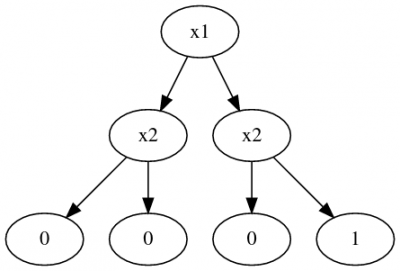
\includegraphics[width=5cm, interpolate]{rsc/bt1.png}
                \parbox{\linewidth}{\captionof{figure}{\centering Tree from Assignment Brief}} 

                \columnbreak
                \null \vfill

                \begin{tabular}[t]{ c|c|c }
                    \texttt{x1} & \texttt{x2}   & $f(\texttt{x1},\texttt{x2})$ \\ \hline
                    0           & 0             & \textcolor{red}{0} \\
                    0           & 1             & \textcolor{red}{0} \\
                    1           & 0             & 0 \\
                    1           & 1             & 1
                \end{tabular} \null \vspace{2ex}
                \parbox{\linewidth}{\captionof{figure}{\centering Truth Table for $f$}} 
            \end{center}
        \end{multicols}
    \end{minipage}

    The second simplification method seeks for similar redundancy in variables, but instead looks for redundacy higher up in the tree. Consider the following tree diagram, also from the assignment brief, and notice that the value of \texttt{x1} has no influence on the final output of the logic function.
    In the truth table for the function, below, notice how the sections above and below the double horizontal line are identical, this means that the output of the function is independent of \texttt{x1} and it can be purged from the tree. Note that the nodes involving variable \texttt{x3} from the brief were simplified using the previous method to reach this stage. This time, the simplification itself involves discarding one side of the tree, and orphaning the intermediate node on the side of the tree that was kept. In this case, \texttt{x2} is orphaned, and \texttt{0} and \texttt{1} from the side that was kept become \texttt{x1}'s children.
    
    \begin{minipage}{\linewidth}
        \begin{multicols}{2}
            \begin{center} \null \vfill
                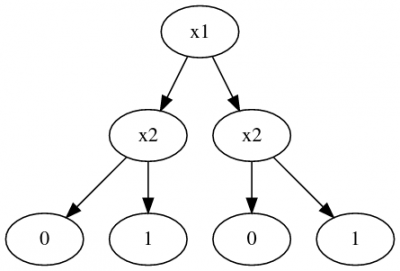
\includegraphics[width=5cm, interpolate]{rsc/bt2.png}
                \parbox{\linewidth}{\captionof{figure}{\centering Tree from Assignment Brief}}

                \columnbreak
                \null \vfill

                \begin{tabular}[t]{ c|c|c }
                    \texttt{x1} & \texttt{x2}   & $f(\texttt{x1},\texttt{x2})$ \\ \hline
                    0           & 0             & 0 \\
                    0           & 1             & 1 \\ \hline\hline
                    1           & 0             & 0 \\
                    1           & 1             & 1
                \end{tabular}  \null \vspace{2ex}
                \parbox{\linewidth}{\captionof{figure}{\centering Truth Table for $f$}}
            \end{center}
        \end{multicols}
    \end{minipage}

    \pagebreak

    Consider the following worked example using the boolean function: \[f(\texttt{x1},\texttt{x2},\texttt{x3})=(A+B)\cdot\overline{C}=\sum\left(2,4,6\right)\] \vspace{-6ex}
    \begin{center}
        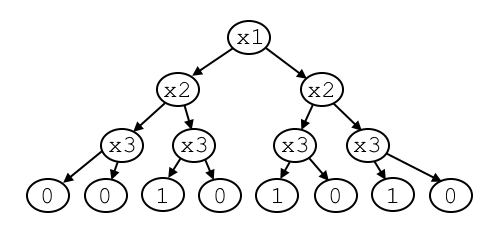
\includegraphics[width=7.5cm, interpolate]{rsc/bt3.png}
        \parbox{\linewidth}{\captionof{figure}{\centering Binary Tree Representing $f$}}
    \end{center} \vspace{-3ex}
    Firstly, an empty tree of depth 3 is constructed. That is to say that all leaves have value 0. Then, leaves at the end of branches representing minterms 010, 100 and 110 are set to 1.

    Simplification now begins, first checking for adjacency. The first two leaves from the left share a parent and their values, so their parent's value is set to the child's value. On the second pass, there is no more simplification, so the next simplification method is applied.

    It can be seen that the four right hand leaves are independent of \texttt{x2} and so that variable can be eliminated  in that path, this is the second simplification method. The next pass does not simplify further and the final version is given below.
    \begin{center} \vspace{-3ex}
        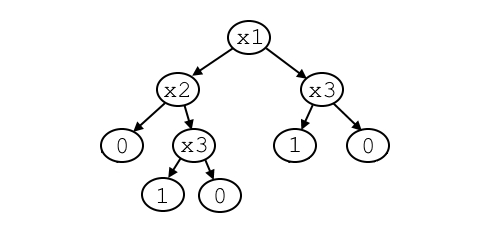
\includegraphics[width=7.5cm, interpolate]{rsc/bt4.png}
        \parbox{\linewidth}{\captionof{figure}{\centering Simplified Binary Tree Representing $f$}}
    \end{center}

    \newpage

    \section{Testing and Evaluation} \vspace{-3ex}
    An important part of testing is being able to visualise the tree. Quite some time was spent attempting to create a function that would print the tree, but I ended up simply using VS~Code's tooltips when hovering over variables in debug mode. This allowed me to inspect the state of the tree, without writing a printing function, although it would still have been a luxury to have such a function.

    I began writing the program using the provided examples as a basis of what kind of simplification to perform, so tested those function first, and after some work, reduced as much as they did in the examples provided.

    Writing the actual simplification methods was not too complicated, but and example of an optimisation that was found was regarding the loops that govern how many times the simplification methods are applied.

    Initially, the methods would run as many times as there are layers as this is theoretically the most times that they could be run. For instance, consider a tree where all leaf values are \texttt{1} with three variables. The first simplfication method (adjacency) would simplify this to simply \texttt{1} after three simplification passes. However, at the time I failed to consider the fact that if the simplification is unsuccessful once, there is no point trying again. This can save quite a lot of time as the simplification functions are recursive and for bigger trees can significantly slow down execution.
    
    To gain an idea of the performance of the simplification, a speadsheet was used to graph the reduction ratio. Given a number $n$ of variables, the full tree will contain $2^{n+1}-1$ nodes. This follows from the fact that a tree with one variable has 3 nodes, and adding a variable increases the tally by 4, then 8 and so on. With a fixed number of minterms, for instance 4, the reduction ratio increases as variables are added. This is due to the fact that adding variables, and not minterms, increases the probability of dependence between the minterms and hence simplification opportunity. The following graph was generated by getting 4 random paths for minterms with 3, 4, 5, 6 and 7 variables.
    \begin{center} \vspace{-3ex}
        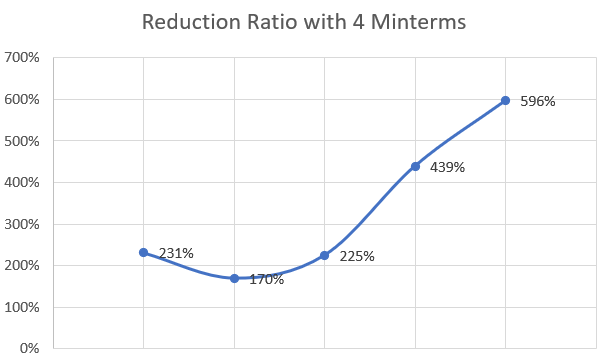
\includegraphics[width=7.5cm, interpolate]{rsc/stats.png}
        \parbox{\linewidth}{\captionof{figure}{\centering Graph Showing Reduction Ratio with 4 Minterms from 3 Variables to 7 Variables}}
    \end{center}

    \section{Closing Words}
    Before closing, let's reconsider the inital decision that was made to simplify the tree after constructing the full version. Using this paradigm, signifcant nodal simplification has been achieved, especially when the number of minterms is smaller than the number of variables, as our Excel adventure demonstrated. However, doing this implies that there is one aspect that prevents further simplification, and that is the fact that the order of variables is set in stone. That is to say that \texttt{x2} cannot be the parent node of \texttt{x1} for example. Of course, this means that there will be scenarios where better simplification could be achieved if there was a way of finding which variable was the best to select when creating children. The \texttt{eval\_bt} function is flexible as the index corresponding to the variable number will be read to decide to go left or right.

    However, even considering the potential for greater simplification, there comes a point where one must consider tradeoffs. This report has to be short. My explaination of a simple alogrithm barely fits into the size constraint, and thoroughly explaining a much more complicated alogrithm would be challenging in this environment.
\end{document}